\documentclass[12pt, xcolor=beamer,table,usenames,dvipsnames, ignorenonframetext, ngerman,t]{beamer}
\usetheme{Frankfurt}
\usecolortheme{dove}
\usepackage{appendixnumberbeamer}
%\setbeamersize{text margin left=20pt,text margin right=20pt,}

\beamertemplatenavigationsymbolsempty 
\setbeamertemplate{headline}{}
\setbeamertemplate{itemize item}{\textbullet}

\addtobeamertemplate{navigation symbols}{}{
	\ifnum\insertframenumber>\inserttotalframenumber%
	\relax
	\else%
	\usebeamerfont{footline}%
	\usebeamercolor[fg]{footline}%
	\hspace{1em}%
	\insertframenumber
	\fi%
}
\addtobeamertemplate{frametitle}{\vspace*{.5cm}}{\vspace*{.5cm}}

\setbeamercolor{footline}{fg=black}
\usepackage{soul}
\makeatletter
\let\HL\hl
\renewcommand\hl{%
	\let\set@color\beamerorig@set@color
	\let\reset@color\beamerorig@reset@color
	\HL}

\usepackage{tipa}
\usepackage{tikz}
\usetikzlibrary{shapes.geometric, arrows}
\mode<presentation>

  \setbeamercovered{invisible}
\usepackage{multicol}
\usepackage[english]{babel}
\usepackage[latin1]{inputenc}
\usepackage{times}
\usepackage[T1]{fontenc}
\usepackage{ulem}
\usepackage{tipa}
\usepackage{qtree}
\usepackage{phonrule}
\usepackage{graphicx}
\usepackage{apacite}
\usepackage{xcolor}
\setlength\parindent{0pt}
\usepackage{natbib}
\usepackage{tikz}
\usetikzlibrary{arrows.meta}
\usepackage{tcolorbox}
\tcbuselibrary{raster}

\newcommand{\bluecheck}{}%
\DeclareRobustCommand{\greencheck}{%
	\tikz\fill[scale=0.6, color=ForestGreen]
	(0,.35) -- (.25,0) -- (1,.7) -- (.25,.15) -- cycle;%
}

\title{A-maze of Natural Stories: Texts are comprehensible using the Maze task}
\author{Veronica Boyce, Roger Levy}
\date{AMLaP 2020}


\begin{document}

\begin{frame}{ }
\vskip 6em

\begin{center}
{\LARGE A-maze of Natural Stories:}

\smallskip

{\Large Texts are comprehensible using\\ \smallskip the Maze task}

\bigskip

{\large Veronica Boyce, Roger Levy}

\bigskip

{\large AMLaP 2020}

\begin{tikzpicture}[remember picture,overlay]
\node[xshift=-1.8cm,yshift=-1cm] at (current page.east) {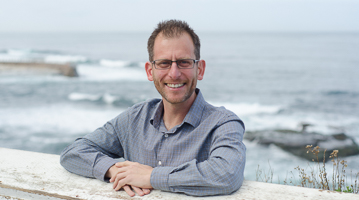
\includegraphics[clip, trim=.1cm 0cm .2cm 0cm,width=.2\textwidth]{roger.jpg}};
\end{tikzpicture}

\begin{tikzpicture}[remember picture,overlay]
\node[xshift=2.5cm,yshift=-1.5cm] at (current page.north west) {
\includegraphics[width=.3\textwidth]{cpl_header.png}};
\end{tikzpicture}



\end{center}
\end{frame}

%\begin{frame}{Incremental processing methods}
%\pause
%Want a measure of processing difficulty\pause
%
%Assume that longer RT = more difficulty \pause
%\smallskip
%\begin{center}
%{\large How to measure RT?}
%\end{center}
%\end{frame}
\begin{frame}{Incremental processing methods}
	\pause
{\large Common ways to measure RT}
\begin{columns}[t]\pause
	\begin{column}{.5\textwidth}
		\begin{center}
			\textbf{\large Eye-tracking}
			
			\medskip
			
			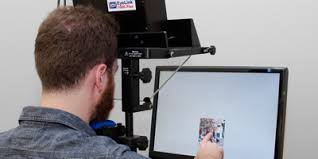
\includegraphics[width=.9\textwidth]{../eye-tracker.jpeg}
			\pause
		\end{center}
	\end{column}
	\begin{column}{.5\textwidth}
		\begin{center}
\textbf{\large Self-paced reading}

\medskip

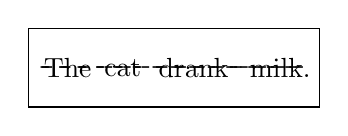
\begin{tikzpicture}
\draw (-.5,-.5) rectangle (3.2,.5);
\onslide<4>{\node at (0,0) {The};}
\onslide<4>{\node at (1.7,0) {- - - - - - - - - - -};}
\onslide<5>{\node at (0,0) {- - - };}
\onslide<5>{\node at (.7,0) {cat};}
\onslide<5>{\node at (2,0) {- - - - - - - - };}
\onslide<6>{\node at (0.3,0) {- - - - - - };}
\onslide<6>{\node at (1.6,0) {drank};}
\onslide<6>{\node at (2.6,0) {- - - -};}
\onslide<7->{\node at (.9,0) {- - - - - - - - - - -};}
\onslide<7->{\node at (2.7,0) {milk.};}
\end{tikzpicture}
\end{center}
\end{column}
\end{columns}
\bigskip
\onslide<8->{Different methods have different trade-offs}
\end{frame}

\begin{frame}[c]{An alternative: Maze}


\centering

\bigskip 

\tikzset{
	font={\fontsize{14pt}{12}\selectfont}}

\begin{tikzpicture}
\onslide<1-2>{\node  (c) at (-1,.5) {The};}
\onslide<1-2>{\node  (d) at (1,.5) {x-x-x};}
\onslide<3-4>{\node  (c) at (-1,.5) {upon};}
\onslide<3-4>{\node  (d) at (1,.5) {dog};}
\onslide<5-6>{\node  (c) at (-1,.5) {revise};}
\onslide<5-6>{\node  (d) at (1,.5) {chased};}
\onslide<7-8>{\node  (c) at (-1,.5) {the};}
\onslide<7-8>{\node  (d) at (1,.5) {wish};}
\onslide<9-10>{\node  (c) at (-1,.5) {mitigate.};}
\onslide<9-10>{\node  (d) at (1,.5) {squirrel.};}
\onslide<2,8>{\node[ultra thick, draw=blue, ellipse, minimum width=60pt, minimum height= 25pt,align=center] at (c) {};}
\onslide<4,6,10>{\node[ultra thick, draw=blue, ellipse, minimum width=60pt, minimum height= 25pt,
align=center] at (d) {};}
\end{tikzpicture}
\end{frame}

\begin{frame}{An alternative: Maze}
\vskip -1em
{\small(Forster et al. 2009; Witzel et al. 2012)}
	\vskip -1em
\begin{columns}
	\begin{column}{0.5\textwidth}
		\begin{center}
		\textbf{\large G-maze}\\
		`Grammatical' choices\\
		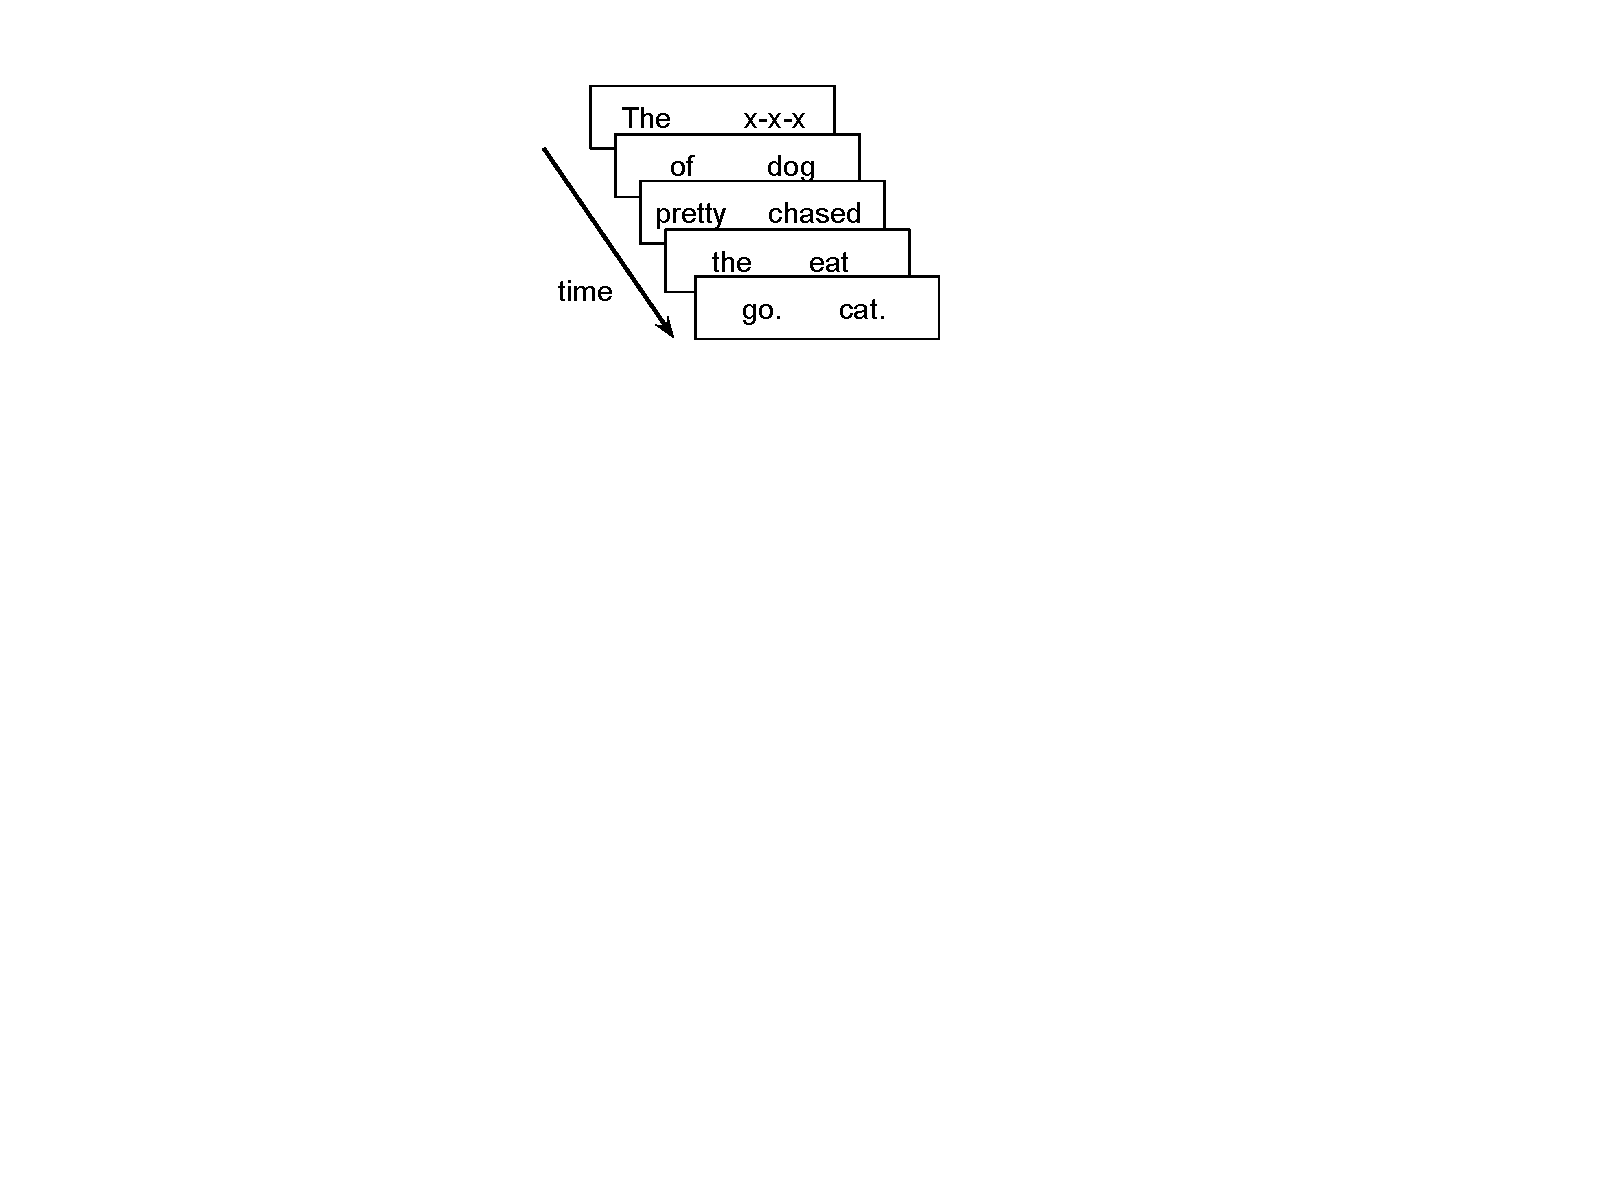
\includegraphics[clip, trim=9cm 14cm 11cm 1cm,width=.9\textwidth]{../gmaze.pdf}
		\end{center}
	\pause
	\end{column}
	\begin{column}{0.5\textwidth} 
		\begin{center}
		\textbf{\large L-maze}\\
		`Lexical' choices\\
			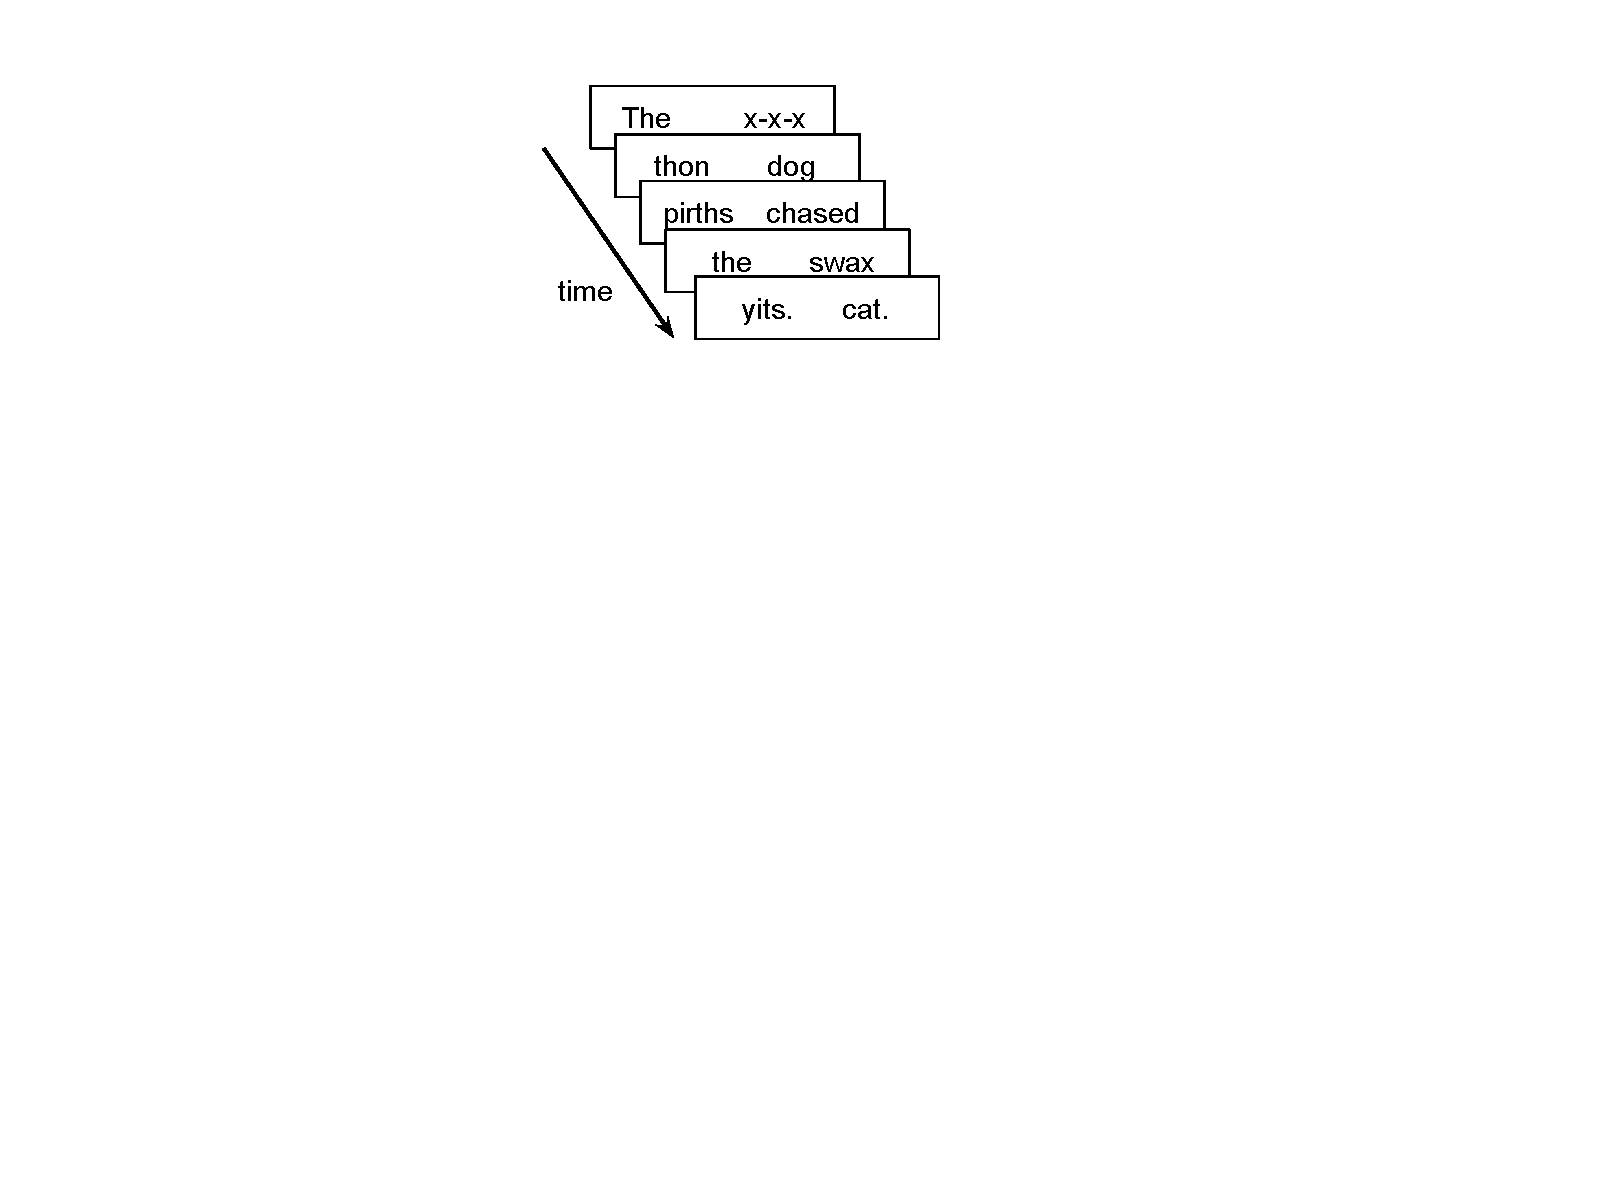
\includegraphics[clip, trim=9cm 14cm 11cm 1cm,width=.9\textwidth]{../lmaze.pdf}
		\end{center}
	\end{column}
\end{columns}

\medskip
\pause
Sentence ends if a mistake is made.
\pause

Claim: forces incremental processing (no spillover)
% Compelling results especially for G-maze, but 
% was run in the lab, and generating G-maze materials is a huge amount of work
\end{frame}

\begin{frame}{Maze Made Easy}
	
	Can we use Maze instead of web SPR?\pause
	
	\medskip
	
	Needs some tweaks:\pause
	\begin{itemize}
		\item Run on web \pause
		\item Easily generate distractors \pause
		\item Work for multi-sentence items
	\end{itemize} 
	
\end{frame}

\begin{frame}{Run on web}
	
	\pause
	Wrote an Ibex module \pause
	
	\begin{center}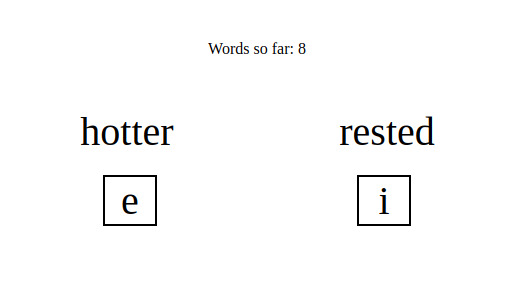
\includegraphics[width=.7\textwidth]{screenshot.png} \end{center}\pause

 Replicated Witzel et al. (2012) results (Boyce et al. 2020)
\end{frame}
%
\begin{frame}{Maze Made Easy}
	
	Can we use Maze instead of web SPR?
	
	\medskip
	
	Needs some tweaks:
	\begin{itemize}
		\item Run on web \greencheck
		\item Easily generate distractors
		\item Work for multi-sentence items %this part incidentally makes it easy to do exclusions, and might help with data loss, but we'll talk about that later
	\end{itemize} 
	
\end{frame}
%
\begin{frame}{Generating distractors}
\pause
Goal: Find a word that can't continue a partial sentence
\begin{itemize}
	\item Ex.  \textit{The dog chased} \pause
	\item Tedious (and hard!) to do by hand
\end{itemize} \pause

What makes something an unacceptable continuation? \pause
\begin{itemize}
	\item Ungrammatical \pause
	\item ...or otherwise really unlikely \pause 
	\item $\approx$ high surprisal 
\end{itemize} \pause

Can we use Neural Language Models?
\end{frame}
%
\begin{frame}{Can we use LMs?}
	\pause
Language models (LMs)
\begin{itemize}
	\item Trained to predict the next word
	\item Given a partial sentence, return probabilities of the next word
\end{itemize}\pause

Run items through LM, choose high surprisal words as distractors

%Add some restrictions:
%\begin{itemize}
%\item Restrict to a list of possible distractors
%\item Only consider length, frequency matches
%\end{itemize}
%	
\end{frame}
%
\begin{frame}{Does it work?} 
\pause
%\vskip -2em
{\large Yes, at least well enough.} \pause
\begin{itemize}
	\item Sometimes generates plausible distractors. \pause
	\item A-maze results comparable with G-maze {\small(Boyce et al 2020, Sloggett et al 2020)}
\end{itemize} 
\end{frame}

\begin{frame}{Does it work?} 
	%\vskip -2em
		\small
	From ``Maze Made Easy'' (Boyce et al 2020)
	\medskip
	
	\centering
	
	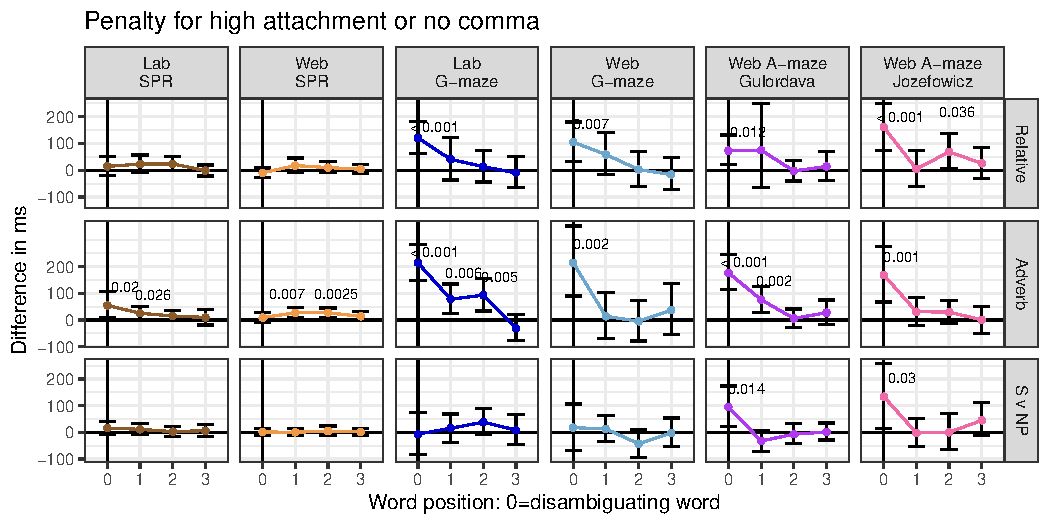
\includegraphics[width=\textwidth]{../spr_g_amaze.pdf}
	
		{\footnotesize Error bars: 95\% CI}

\end{frame}
%
\begin{frame}{Maze Made Easy}
	
	Can we use Maze instead of web SPR?
	
	\medskip
	
	Needs some tweaks:
	\begin{itemize}
		\item Run on web \greencheck
		\item Easily generate distractors \greencheck
		\item Work for multi-sentence items 
	\end{itemize} 
	
\end{frame}
%
%
\begin{frame}{Long items}

Want to run multi-sentence items. \pause

Problem: Errors terminate sentences. \pause
\begin{itemize}
	\item Treat whole story as a unit: \pause Few participants make it to the end. \pause
	\item Treat each sentence as a unit: \pause Some participants miss key context. \pause
\end{itemize}

What if after an error, participants corrected errors and the sentence continued?
	
\end{frame}
%
\begin{frame}[c]{Maze with Error Correction}
\centering
\tikzset{
	font={\fontsize{14pt}{12}\selectfont}}

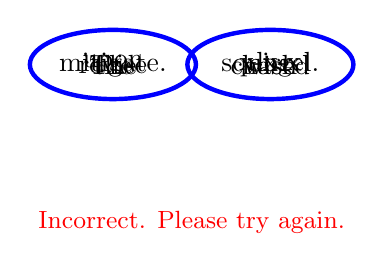
\begin{tikzpicture}
\onslide<1-2>{\node  (c) at (-1,.5) {The};}
\onslide<1-2>{\node  (d) at (1,.5) {x-x-x};}
\onslide<3-4>{\node  (c) at (-1,.5) {upon};}
\onslide<3-4>{\node  (d) at (1,.5) {dog};}
\onslide<5-8>{\node  (c) at (-1,.5) {revise};}
\onslide<5-8>{\node  (d) at (1,.5) {chased};}
\onslide<9-10>{\node  (c) at (-1,.5) {the};}
\onslide<9-10>{\node  (d) at (1,.5) {wish};}
\onslide<11-12>{\node  (c) at (-1,.5) {mitigate.};}
\onslide<11-12>{\node  (d) at (1,.5) {squirrel.};}
\onslide<2,6,10>{\node[ultra thick, draw=blue, ellipse, minimum width=60pt, minimum height= 25pt,align=center] at (c) {};}
\onslide<4,8,12>{\node[ultra thick, draw=blue, ellipse, minimum width=60pt, minimum height= 25pt,
	align=center] at (d) {};}
\onslide<7,8>{\node[text=red] at (0,-1.5) {\small Incorrect. Please try again.};}
\end{tikzpicture}

\end{frame}

\begin{frame}{Maze with Error Correction}

\begin{columns}
	\begin{column}{0.4\textwidth}
		\begin{center}
		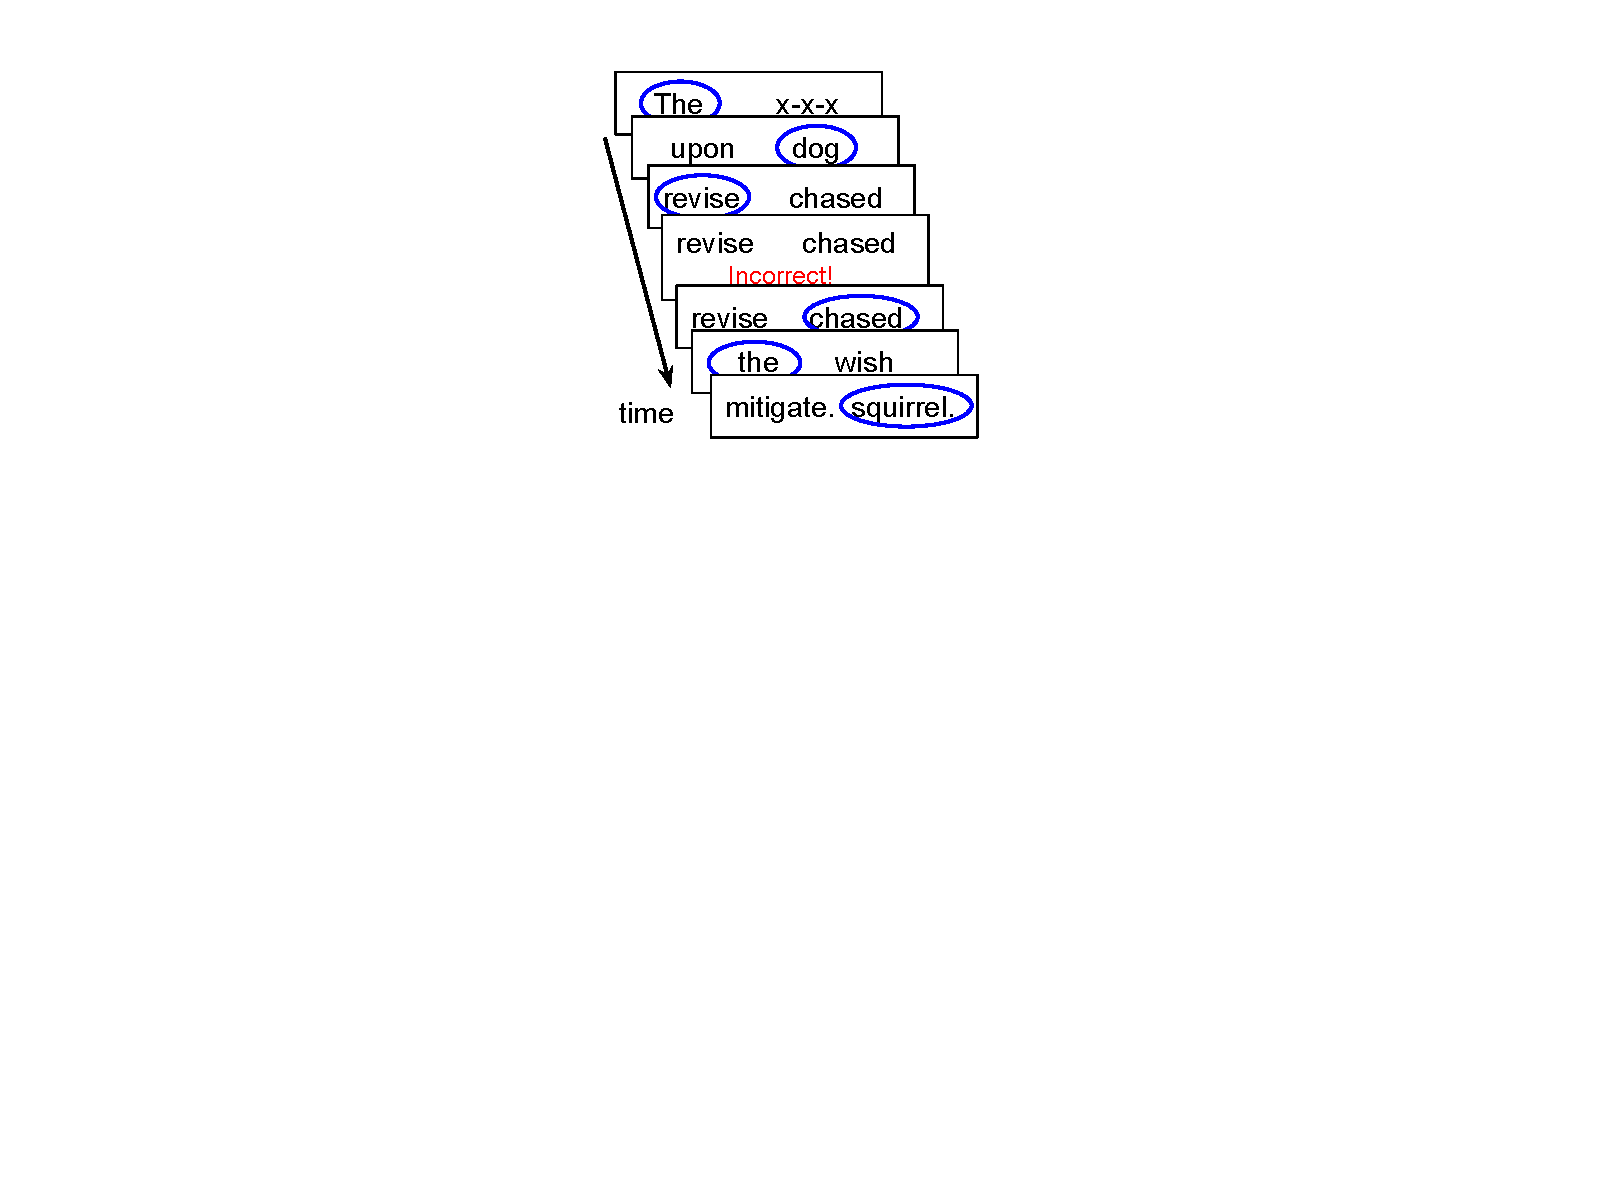
\includegraphics[clip, trim=9cm 12.5cm 10cm 1cm,width=\textwidth]{../maze_diagram.pdf}
		\end{center}
		
	\end{column} \pause 
	\begin{column}{0.6\textwidth} 
		\begin{center}
			\begin{itemize}
				\item Can be toggled in Ibex Maze \pause
				\item Long materials feasible \pause
				\item Have all the data \pause
				\item Compensates for bad distractors
			\end{itemize}
		\end{center}
	\end{column}
\end{columns}
\end{frame}
%

\begin{frame}{Maze Made Easy}
	
	Can we use Maze instead of web SPR?
	
	\medskip
	
	Needs some tweaks:
	\begin{itemize}
		\item Run on web \greencheck
		\item Easily generate distractors \greencheck
		\item Work for multi-sentence items \greencheck ? 
	\end{itemize} 
	
\end{frame}
%%So now that I've explained the method, going to switch over to current experiment & what we hoped to get from it
%
\begin{frame}{Current experiment}
	Various open questions to address \pause
	\begin{itemize}
		\item Will people read long texts in Maze? \pause
		\item Will they comprehend what they read? \pause
		\item Does error correction Maze work? \pause
		\item Do we get predictability effects? 
	\end{itemize}
\end{frame}

\begin{frame}{Natural Stories}
Natural stories corpus (Futrell et al. 2017) \pause
\begin{itemize}
	\item 10 stories, each about 1000 words \pause
%	\item Some unusual constructions, but read fluently \pause
	\item 6 comprehension questions per story
\end{itemize}

\end{frame}

\begin{frame}{Natural Stories}

\begin{small}Tulip mania was a period in the Dutch Golden Age during which contract prices for bulbs of the recently introduced tulip reached extraordinarily high levels and then suddenly collapsed. At the peak of tulip mania in February sixteen thirty-seven, tulip contracts sold for more than ten times the annual income of a skilled craftsman. It is generally considered the first recorded economic bubble. [...]
\medskip

\pause

Q: When did tulip mania reach its peak?

A: \hspace{3em} 1630's\hspace{3em} 1730's \end{small}

%HARD mode 

\end{frame}

\begin{frame}{Participant accuracy}
100 participants from MTurk each read 1 story (20 minutes) \pause
\begin{center}
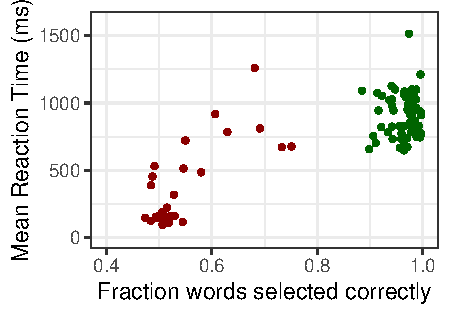
\includegraphics[width=.8\textwidth]{../error.pdf}
\end{center}
\end{frame}

\begin{frame}{Comprehension questions}
\begin{center} \pause
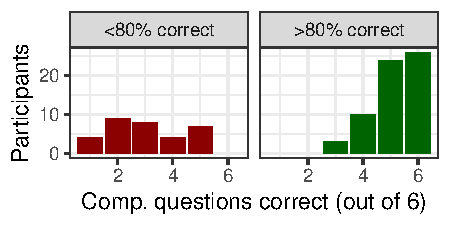
\includegraphics[width=.8\textwidth]{../comp.pdf}
\end{center}
% exclusion options: use comprehension checks as participant filter. Here we can use overall accuracy as the "paying attention" filter. Don't have to worry about how to write good comprehension questions. May still need to do RT exclusions for double-presses or getting distracted. 
\end{frame}


%HERE%
\begin{frame}{Surprisal Effects}
\large{Is RT linear in terms of surprisal?}\pause
\medskip

Estimate surprisal from 3 models:
\begin{itemize}
	\item smoothed 5-gram
	\item LSTM-RNN (Gulordava et al. 2018)
	\item Transformer-XL (Dai et al. 2019)
\end{itemize}

\pause

Fit GAMs
\begin{itemize}
	%\item Limit to single-token words
	\item Fit to both current and past word surprisal
	\item Include frequency, length as predictors
\end{itemize}

\end{frame}

\begin{frame}{Surprisal Effects}
	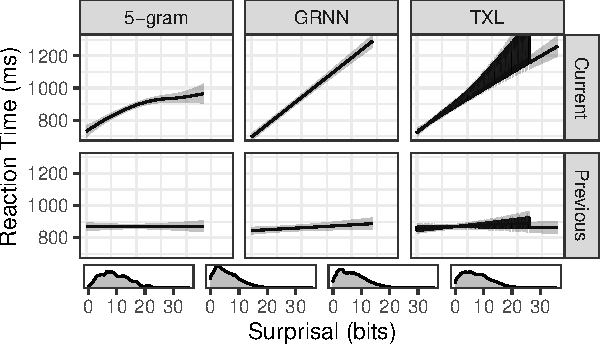
\includegraphics[width=.9\textwidth]{../gam.pdf}	
\end{frame}


\begin{frame}{Surprisal Effects}
	\vskip -2em
	Linear Models \\ 
	\pause
	
	\begin{small}
		\begin{tabular}{l|r|r|r}
			\hline
			&5-gram & GRNN & TXL\\
			\hline
			Intercept & \textbf{865.3} & \textbf{871.1} & \textbf{870.8} \\ 
			Surprisal & \textbf{11.7}  & \textbf{23.7} & \textbf{18.5}  \\ 
			Frequency & -2.9  & 2.9  & 0.4  \\ 
			Length & \textbf{20.5} & \textbf{18.5}  & \textbf{21.4} \\ 
			Surprisal:Length & \textbf{-2.0}  & \textbf{-1.8}  & \textbf{-1.4} \\
			Freq:Length & -1.0  & -0.1 & 0.2  \\ 
			\hline
			Past Surprisal & 1.6  & \textbf{2.7} & 0.8 \\ 
			Past Freq & 2.6  & 1.9  & 1.2  \\ 
			Past Length & \textbf{-4.8}  & \textbf{-6.6 }&\textbf{ -5.2} \\ 
			Past Surp:Length & -0.2 & \textbf{-0.9} & -0.6  \\ 
			Past Freq:Length & -1.0  & \textbf{-1.8 }&   \textbf{-1.5}  \\ 
			\hline
		\end{tabular}
	
	Surprisal in bits, Length in characters, \\
	Frequency in $log_2$ occurrences/billion words
	\end{small}

\end{frame}
\begin{frame}{Surprisal Effects}
	Takeaways: \pause
	\begin{itemize}
		\item Minimal frequency effects (consistent with Shain 2019) \pause
		\item Large effects of Length, Surprisal \pause
		\item Very little spillover \pause
	\end{itemize}
%	
	Model comparison: GRNN is best, but TXL complementary
\end{frame}

\begin{frame}{Why such large effects?}
	\pause
	Bayesian Reader (Norris 2006): Look at words long enough to ID with some threshold of certainty \pause
	
Possible mechanisms for difference: \pause
\begin{itemize}
	\item Higher threshold \pause 
	\item Fewer available resources for processing \pause
	\item Presence of second word 
\end{itemize}

\end{frame}

\begin{frame}{Conclusion}
	
	\pause
	
Consider A-maze! 
\begin{itemize}\pause
	\item Documentation:  \textcolor{ForestGreen}{vboyce.github.io/Maze} \pause
	\item Versatile \pause
	\item Low spillover \pause 
\end{itemize}

Natural Stories A-maze: \pause 
\begin{itemize}
	\item Participants comprehend what they read \pause
	\item Find linear, large surprisal effects
\end{itemize}

\end{frame}

\appendix

\begin{frame}
	\centering
	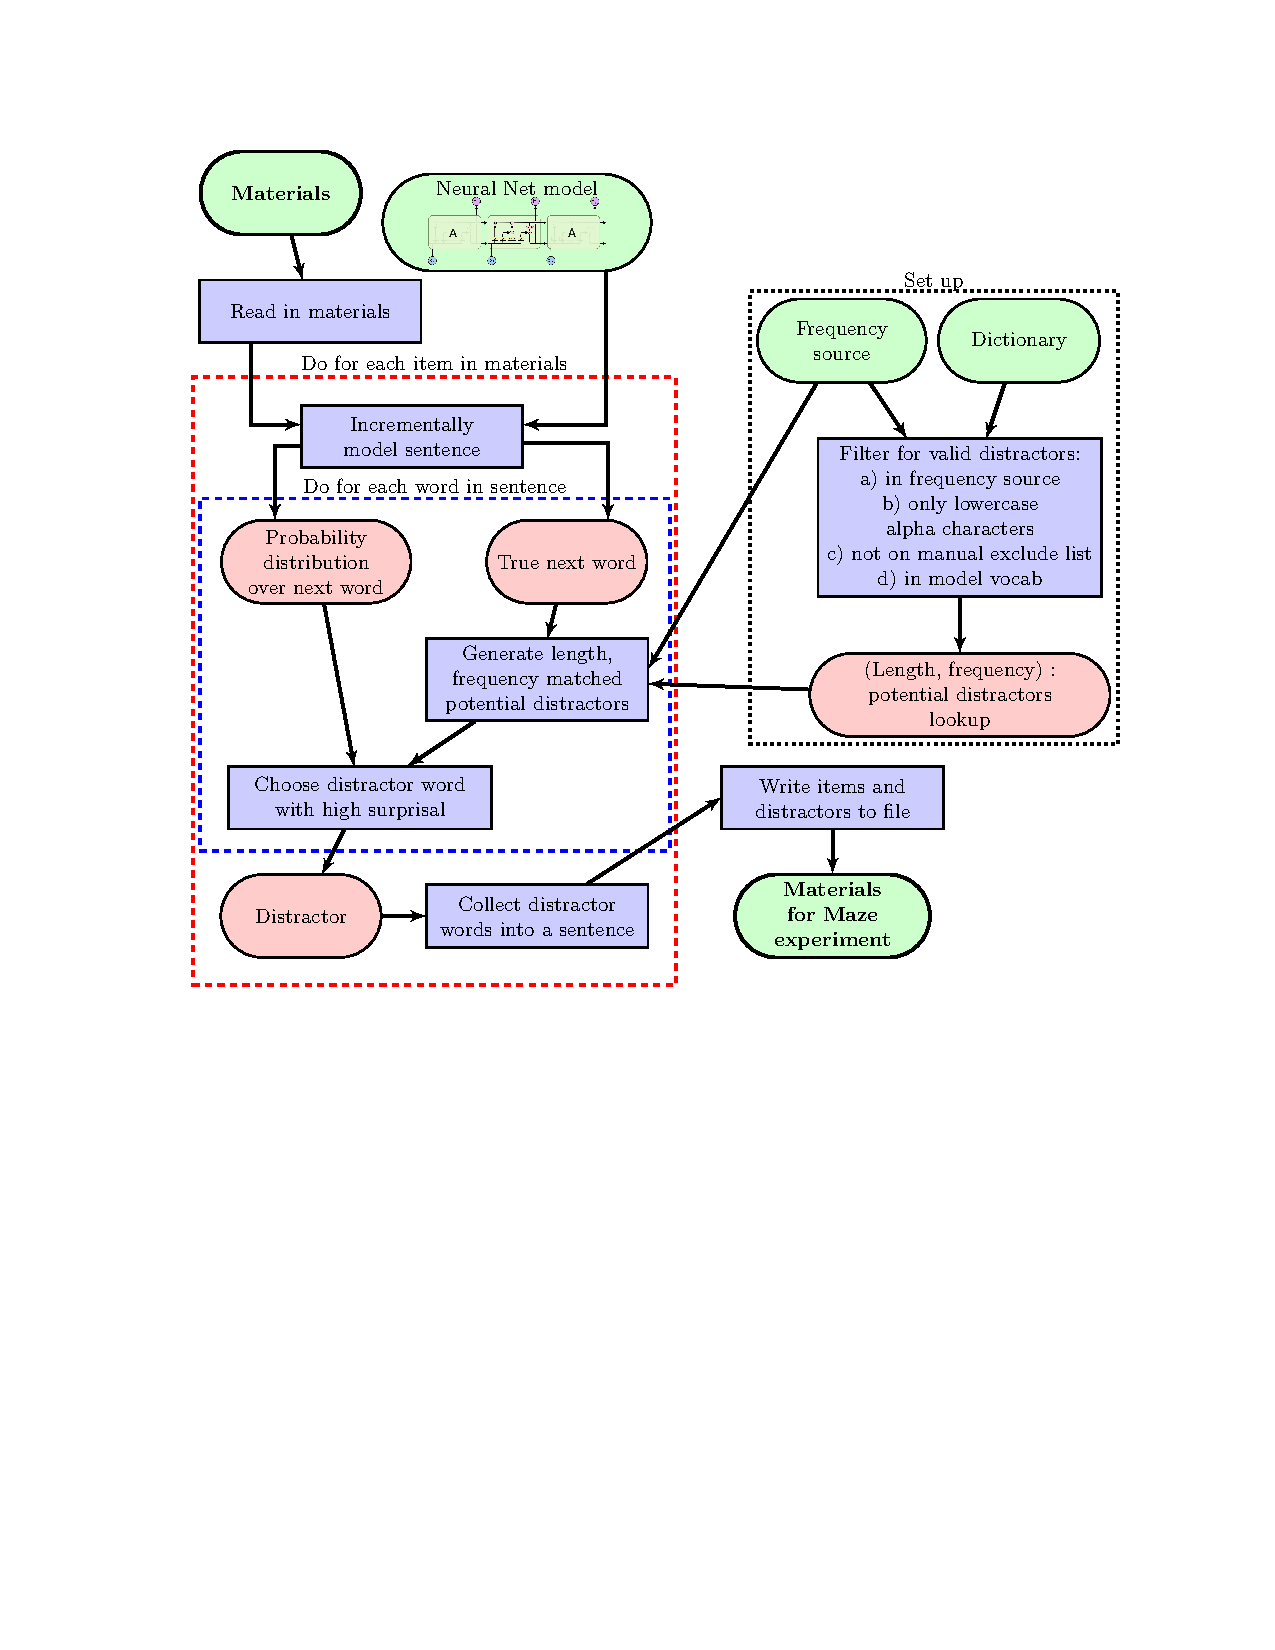
\includegraphics[clip, trim=3.25cm 5cm 2.5cm 2.5cm,width=.9\textwidth]{../flow_2.pdf}
\end{frame}



\begin{frame}{Caveats}
	
	{\large Definitely some bad distractors}
	\begin{table}
		
		
		\begin{tabular}{rlll}
			Prefix & Correct & Distractor & Error Rate \\
			\hline
			\hline
			Gulordava&&&\\
			\hline
			The & niece & cooks & 44\%\\
			The swimmer & disappointed & propositions & 30\%\\
			The & semester & steroids & 29\%\\
			\hline
			\hline
			Jozefowicz&&&\\
			\hline
			The & husband & authors & 46\%\\
			Jim & listened & survived & 43\%\\
			The & uncle & roads & 42\%\\
			The & knight & saints & 40\%\\
		\end{tabular}
	\end{table}
	
\end{frame}

\begin{frame}{Surprisal Effects}
	GAM if we only exclude mistakes (all participants, post-mistake data)
	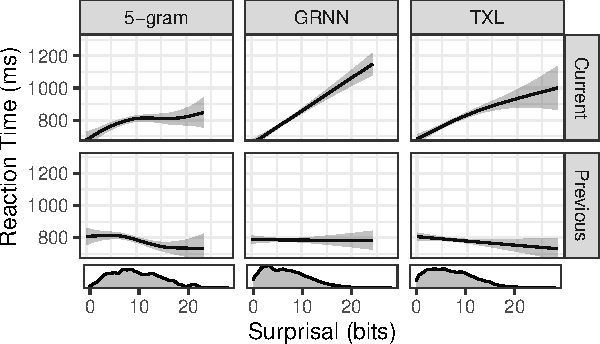
\includegraphics[width=.9\textwidth]{../gam-any.pdf}	
\end{frame}

\begin{frame}{Links}
	
	\textcolor{ForestGreen}{\large Documentation: vboyce.github.io/Maze}
	
	with links to the following:
	\begin{itemize}
		
		\item A-maze code: github.com/vboyce/Maze
		
		\item Web-maze code: github.com/vboyce/Ibex-with-Maze
		
		\item Sample task: syntaxgym.org:666
		
		\item Paper: psyarxiv.com/b7nqd/
	\end{itemize}
\end{frame}


\begin{frame}{Matching distractors}
	If unspecified: Match by position
	\begin{itemize}
		\item The son of the lady who politely introduced \sethlcolor{green} \hl{herself}\sethlcolor{pink} / \hl{himself} was popular at the party.
	\end{itemize}
	Can specify labels for each word to pair (within item)
	\begin{itemize}
		\item The cat who the dog scared hid in a box.\\pre-1 pre-2 who art noun verb main-verb post-1 post-2 post-3
		\item The dog who scared the cat sniffed around the couch.\\ pre-1 pre-2 who verb art noun main-verb post-1 post-2 post-3
	\end{itemize}
\end{frame}

\end{document}

